\documentclass[10.5pt]{article}
\usepackage[letterpaper, margin=0.6in, top=0.5in, bottom=0.5in]{geometry}
\usepackage{amsmath,amssymb,amsthm}
\usepackage{fancyhdr}
\usepackage{xcolor}
\usepackage{tikz}
\usepackage{enumitem}
\usepackage{tcolorbox}
\usepackage{hyperref}

\definecolor{chalkblue}{RGB}{0, 105, 185}
\definecolor{chalkred}{RGB}{205, 35, 35}
\definecolor{chalkpink}{RGB}{230, 90, 120}
\definecolor{chalkcyan}{RGB}{15, 160, 190}
\definecolor{chalkgreen}{RGB}{20, 130, 50}
\definecolor{boxbg}{RGB}{252, 252, 254}
\definecolor{boxframe}{RGB}{150, 160, 180}

\pagestyle{fancy}
\fancyhf{}
\renewcommand{\headrulewidth}{0pt}
\renewcommand{\footrulewidth}{0pt}

\setlength{\parindent}{0pt}
\setlength{\parskip}{2.5pt}

\begin{document}

% ==============================================================================
% PAGE 1
% ==============================================================================
\noindent \textbf{\large Math 105L} \hfill \textbf{\large Lecture 9-3}\\[1pt]
{\textbf{\Large Implicit Differentiation II}}\\[-5pt]
\rule{\textwidth}{1.2pt}

\vspace{0.03in}

\textbf{\large Revisit: Comparing Explicit vs.\ Implicit Differentiation}

\begin{itemize}[leftmargin=1.2em, topsep=1pt, itemsep=2pt]
  \item \textbf{Question:} Let's revisit $xy + y = e^x$. What is $\frac{dy}{dx}$? Check that it's the same as what you got previously!
\end{itemize}

\begin{tcolorbox}[colback=boxbg, colframe=boxframe, boxrule=0.8pt, arc=3pt, left=8pt, right=8pt, top=4pt, bottom=4pt]
\textbf{Method 1: Explicit Differentiation (from previous lecture)}\\[2pt]
Solve for $y$ explicitly first: \quad $y(x+1) = e^x \implies y = \frac{e^x}{x+1}$.\\[2pt]
Differentiating via the Quotient Rule:
\[
  \frac{dy}{dx} = \frac{(x+1)\frac{d}{dx}[e^x] - e^x \frac{d}{dx}[x+1]}{(x+1)^2} = \frac{(x+1)e^x - e^x(1)}{(x+1)^2} = \frac{xe^x + e^x - e^x}{(x+1)^2} = \frac{xe^x}{(x+1)^2}.
\]
\end{tcolorbox}

\vspace{0.02in}

\begin{tcolorbox}[colback=boxbg, colframe=boxframe, boxrule=0.8pt, arc=3pt, left=8pt, right=8pt, top=4pt, bottom=4pt]
\textbf{Method 2: Implicit Differentiation (new approach)}\\[2pt]
Treat $y$ as an implicit function of $x$, writing $y = y(x)$:
\[
  x \cdot y(x) + y(x) = e^x.
\]
Differentiate both sides with respect to $x$ using the \textbf{Product Rule} on $x \cdot y(x)$:
\[
  \underbrace{\frac{d}{dx}[x] \cdot y(x) + x \cdot \frac{d}{dx}[y(x)]}_{\text{Product Rule on } x\cdot y} + \frac{d}{dx}[y(x)] = \frac{d}{dx}[e^x]
\]
\[
  1 \cdot y(x) + x \cdot y'(x) + y'(x) = e^x.
\]
Factor out $y'(x)$ to isolate the derivative:
\[
  y'(x)(x + 1) + y(x) = e^x \implies y'(x)(x + 1) = e^x - y(x) \implies y'(x) = \frac{e^x - y(x)}{x + 1}.
\]
\textbf{Verification:} Substitute the original relation $y(x) = \frac{e^x}{x+1}$ into our implicit derivative formula:
\[
  y'(x) = \frac{e^x - \frac{e^x}{x+1}}{x+1} \cdot \frac{x+1}{x+1} = \frac{e^x(x+1) - e^x}{(x+1)^2} = \frac{xe^x + e^x - e^x}{(x+1)^2} = \frac{xe^x}{(x+1)^2}. \quad \checkmark \text{ (Identical!)}
\]
\end{tcolorbox}

\vspace{0.03in}

\textbf{\large The Core Mechanism of Implicit Differentiation}
\begin{tcolorbox}[colback=blue!3!white, colframe=chalkblue, boxrule=0.8pt, arc=3pt, left=8pt, right=8pt, top=4pt, bottom=4pt]
We pretend $y$ is a function of $x$, making expressions like $y^2, y^3, e^y$, etc.\ into compositions $[y(x)]^2, [y(x)]^3, e^{y(x)}$.
We then apply the \textbf{Chain Rule} and \textbf{Product Rule}:
\begin{itemize}[leftmargin=1.2em, topsep=1pt, itemsep=1pt]
  \item $\frac{d}{dx}[y^n] = n y^{n-1} \cdot \frac{dy}{dx}$ \quad (e.g. $\frac{d}{dx}[y^3] = 3y^2 \cdot y'$)
  \item $\frac{d}{dx}[x \cdot y] = 1 \cdot y + x \cdot y'$ \quad (\textbf{Product Rule})
  \item Gather all terms with $y'$ on one side, factor out $y'$, and divide by the coefficient expression.
\end{itemize}
\end{tcolorbox}

\vfill
\noindent \textbf{\small Math 105L} \hfill \textbf{\small Page 2 of 5}

\newpage

% ==============================================================================
% PAGE 2
% ==============================================================================
\noindent \textbf{\large Math 105L} \hfill \textbf{\large Lecture 9-3}\\[1pt]
{\textbf{\Large Implicit Differentiation II --- Practice Questions}}\\[-5pt]
\rule{\textwidth}{1.2pt}

\vspace{0.05in}

\textbf{\large Question 1: Finding Tangent Lines to Algebraic Curves}

\textbf{1. (a) Find the tangent line to $x^2 + xy - y^3 = xy^2$ at the point $(1,1)$.}

\vspace{0.02in}

\begin{minipage}[t]{0.68\textwidth}
  \textbf{Step 1: Write $y$ explicitly as $y(x)$ and differentiate:}
  \[
    x^2 + x \cdot y(x) - [y(x)]^3 = x \cdot [y(x)]^2
  \]
  Differentiating each term with respect to $x$:
  \[
    2x + \big(x \cdot y'(x) + y(x) \cdot 1\big) - 3[y(x)]^2 y'(x) = x \cdot \big(2y(x) y'(x)\big) + 1 \cdot [y(x)]^2
  \]
  \textbf{Step 2: Collect and isolate $y'$ terms:}
  \[
    2x + x y' + y - 3y^2 y' = 2xy y' + y^2
  \]
  \[
    x y' - 3y^2 y' - 2xy y' = y^2 - 2x - y
  \]
  \[
    y'(x - 3y^2 - 2xy) = y^2 - 2x - y
  \]
  \[
    \frac{dy}{dx} = \frac{y^2 - 2x - y}{x - 3y^2 - 2xy}
  \]
\end{minipage}
\hfill
\begin{minipage}[t]{0.29\textwidth}
  \begin{tcolorbox}[colback=yellow!5!white, colframe=orange!80!black, boxrule=0.6pt, arc=2pt, left=4pt, right=4pt, top=4pt, bottom=4pt]
    \textbf{\footnotesize Deriv.\ of $[y(x)]^3$:}
    \begin{itemize}[leftmargin=0.9em, topsep=0pt, itemsep=0pt]
      \item \scriptsize inner: $y(x)$, outer: $u^3$
      \item \scriptsize inner$'$: $y'(x)$, outer$'$: $3u^2$
      \item \scriptsize $\implies 3y^2 \cdot y'$
    \end{itemize}
    \vspace{2pt}
    \textbf{\footnotesize Deriv.\ of $[y(x)]^2$:}
    \begin{itemize}[leftmargin=0.9em, topsep=0pt, itemsep=0pt]
      \item \scriptsize inner: $y(x)$, outer: $u^2$
      \item \scriptsize inner$'$: $y'(x)$, outer$'$: $2u$
      \item \scriptsize $\implies 2y \cdot y'$
    \end{itemize}
  \end{tcolorbox}
\end{minipage}

\vspace{0.05in}

\textbf{Step 3: Evaluate slope at $(x,y) = (1,1)$:}
\[
  m = \left.\frac{dy}{dx}\right|_{(1,1)} = \frac{(1)^2 - 2(1) - 1}{1 - 3(1)^2 - 2(1)(1)} = \frac{1 - 2 - 1}{1 - 3 - 2} = \frac{-2}{-4} = \frac{1}{2}.
\]

\textbf{Step 4: Tangent Line Equation at $(1,1)$:}
\[
  y - y_0 = m(x - x_0) \implies y - 1 = \frac{1}{2}(x - 1) \implies y = \frac{1}{2}x + \frac{1}{2}.
\]

\vspace{0.06in}
\rule{\textwidth}{0.6pt}
\vspace{0.04in}

\textbf{1. (b) Here's a picture of this curve. Plug the point $(0,0)$ and $(1,-1)$ into your expression for $\frac{dy}{dx}$. What do you get? Looking at the graph, what can you say about the slope at those points?}

\begin{minipage}[c]{0.52\textwidth}
  \begin{itemize}[leftmargin=1.2em, topsep=1pt, itemsep=3pt]
    \item \textbf{At point $(0,0)$:}
    \[
      \left.\frac{dy}{dx}\right|_{(0,0)} = \frac{0^2 - 2(0) - 0}{0 - 3(0)^2 - 2(0)(0)} = \frac{0}{0} \quad \text{\textbf{(Indeterminate / Undefined)}}.
    \]
    \textit{Geometric interpretation:} The curve crosses itself at the origin (a node / self-intersection), meaning there are \textbf{two distinct tangent slopes} at $(0,0)$, so $\frac{dy}{dx}$ cannot be uniquely defined single-valuedly.
    
    \item \textbf{At point $(1,-1)$:}
    \[
      \text{Denominator: } 1 - 3(-1)^2 - 2(1)(-1) = 1 - 3 + 2 = 0.
    \]
    When the denominator of $\frac{dy}{dx}$ equals zero (while the numerator is non-zero or approaching limits), the tangent line is \textbf{vertical} ($\frac{dy}{dx} \to \pm\infty$).
  \end{itemize}
\end{minipage}
\hfill
\begin{minipage}[c]{0.45\textwidth}
  \centering
  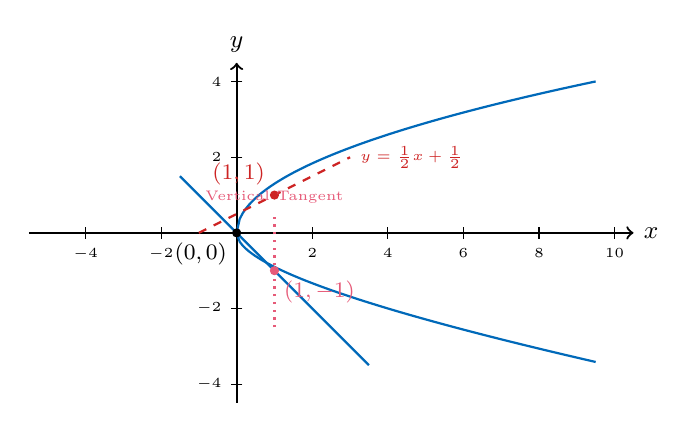
\begin{tikzpicture}[scale=0.48]
    \draw[->, thick] (-5.5,0) -- (10.5,0) node[right] {\small $x$};
    \draw[->, thick] (0,-4.5) -- (0,4.5) node[above] {\small $y$};
    \foreach \x in {-4, -2, 2, 4, 6, 8, 10}
      \draw (\x, 0.15) -- (\x, -0.15) node[below] {\tiny $\x$};
    \foreach \y in {-4, -2, 2, 4}
      \draw (0.15, \y) -- (-0.15, \y) node[left] {\tiny $\y$};
      
    % Branches of curve x^2 + xy - y^3 = x y^2
    \draw[thick, chalkblue, domain=-3.5:1.5, samples=100] plot ({-\x}, {\x});
    \draw[thick, chalkblue, domain=0:9.5, samples=120] plot ({\x}, {sqrt(\x) + 0.3*sqrt(\x)});
    \draw[thick, chalkblue, domain=0:9.5, samples=120] plot ({\x}, {-0.8*sqrt(\x) - 0.1*\x});
    
    % Tangent line at (1,1)
    \filldraw[chalkred] (1,1) circle (3pt) node[above left] {\footnotesize $(1,1)$};
    \draw[chalkred, thick, dashed] (-1, 0) -- (3, 2) node[right] {\tiny $y = \frac{1}{2}x + \frac{1}{2}$};
    
    % Origin point
    \filldraw[black] (0,0) circle (3pt) node[below left] {\footnotesize $(0,0)$};
    % Point (1,-1)
    \filldraw[chalkpink] (1,-1) circle (3pt) node[below right] {\footnotesize $(1,-1)$};
    \draw[chalkpink, thick, dotted] (1,-2.5) -- (1, 0.5) node[above] {\tiny Vertical Tangent};
  \end{tikzpicture}
\end{minipage}

\vfill
\noindent \textbf{\small Math 105L} \hfill \textbf{\small Page 3 of 5}

\end{document}

